\subsection{Inicio de Sesión}

\begin{figure}[H]
    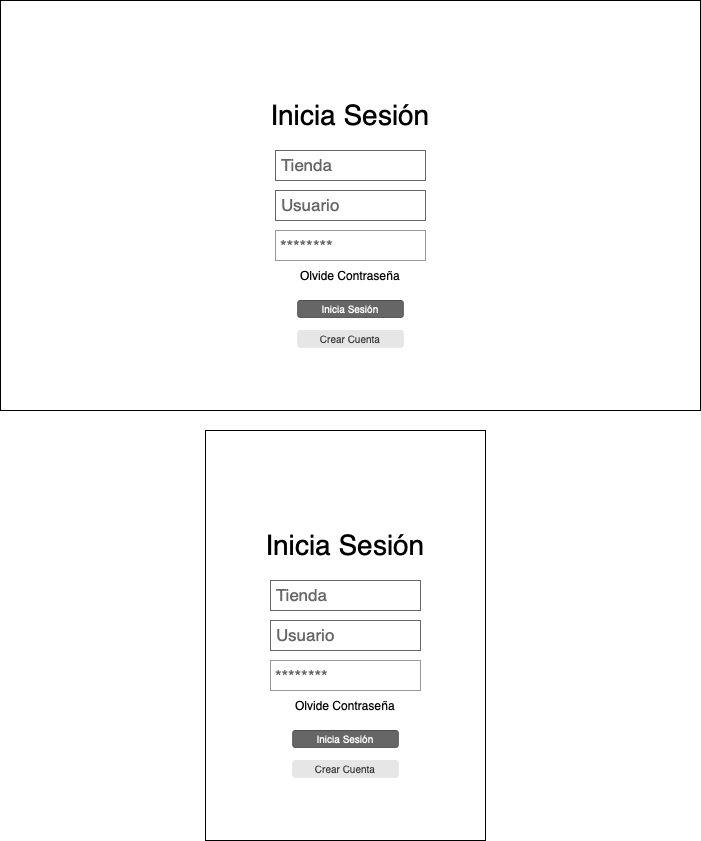
\includegraphics[scale=.4]{images/InicioSesion.png}
    \centering
    \caption{Página de inicio de sesión en web y vista de cliente Android.}
\end{figure}

\subsection{Crear Cuenta}

\begin{figure}[H]
    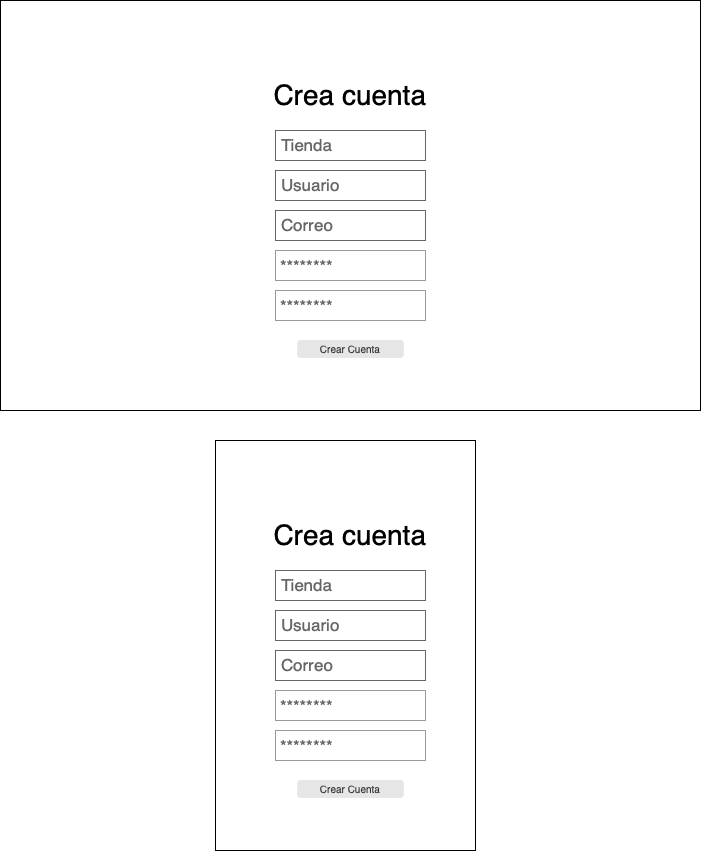
\includegraphics[scale=.4]{images/CreaCuenta.png}
    \centering
    \caption{Página para la creación de una cuenta en web y vista en cliente Android.}
\end{figure}

\subsection{Página de Inicio}

\begin{figure}[H]
    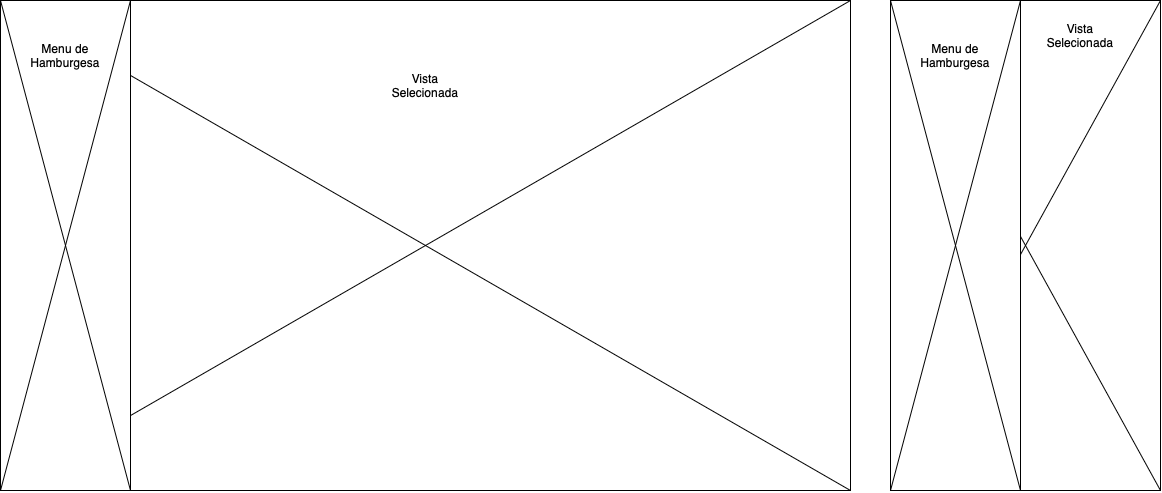
\includegraphics[scale=.4]{images/Inicio.png}
    \centering
    \caption{Página de inicio de la aplicación web y su contraparte en cliente Android.}
\end{figure}

\subsection{Punto de Venta}

\begin{figure}[H]
    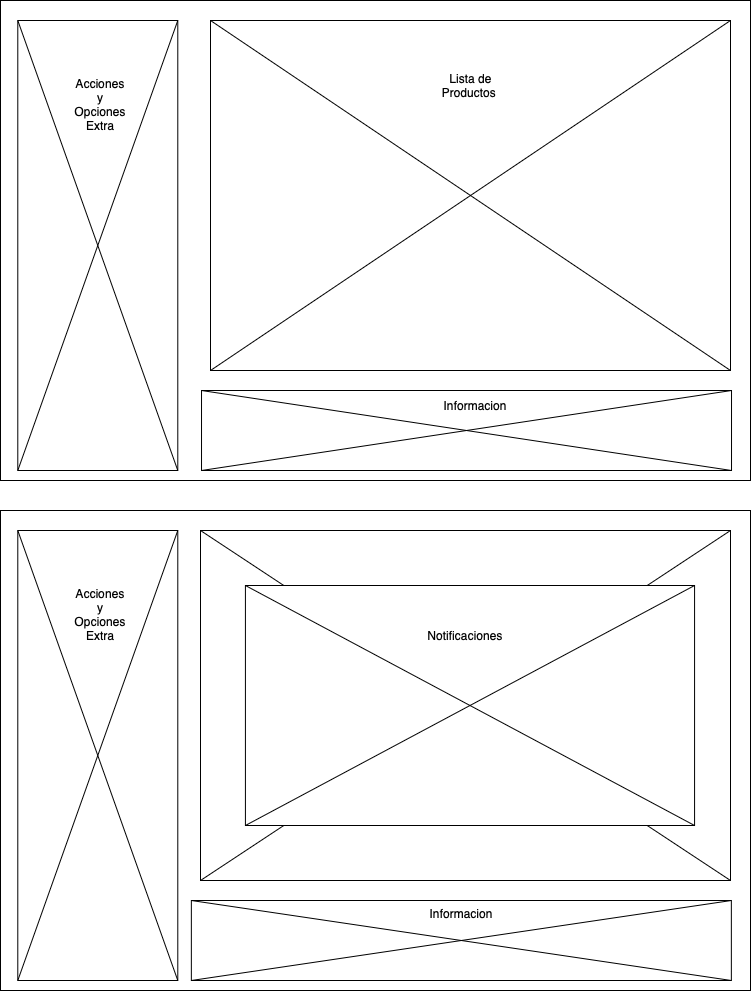
\includegraphics[scale=.4]{images/POS.png}
    \centering
    \caption{Página del punto de venta en web con notificación emergente.}
\end{figure}

\subsection{Administración}

\begin{figure}[H]
    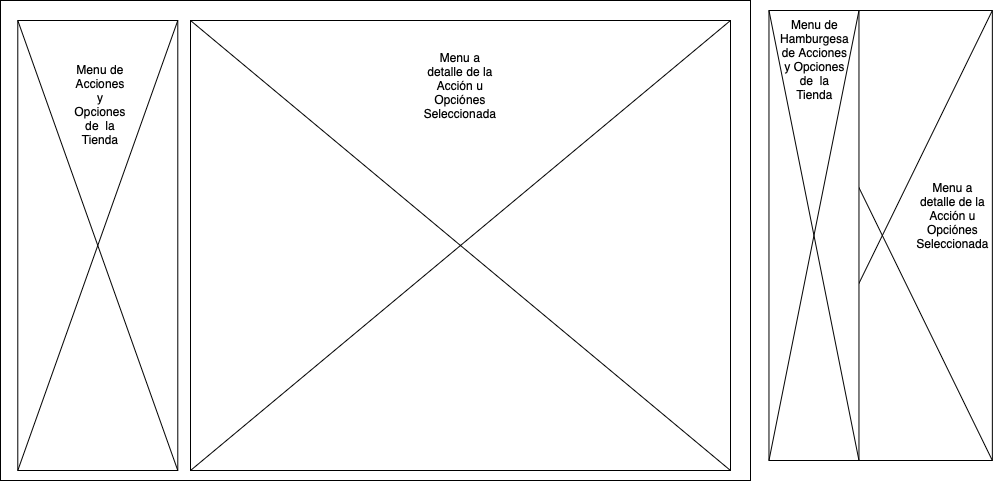
\includegraphics[scale=.4]{images/Administracion.png}
    \centering
    \caption{Página de administración de la tienda en web con su contraparte en el cliente Android.}
\end{figure}

\subsection{Manejo de Inventario}

\begin{figure}[H]
    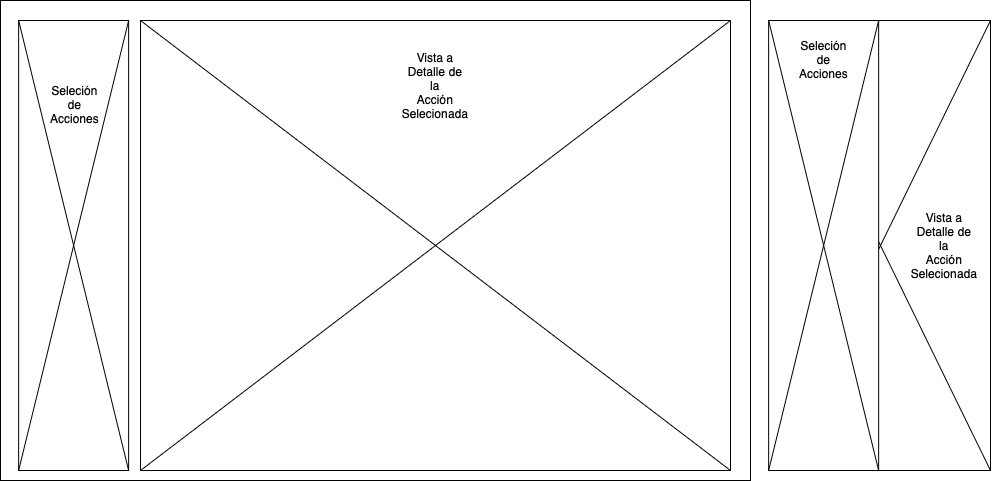
\includegraphics[scale=.4]{images/Inventario.png}
    \centering
    \caption{Página para el manejo del inventario de la tienda en web y en su vista Android.}
\end{figure}

\subsection{Análisis de Datos y Reportes}

\begin{figure}[H]
    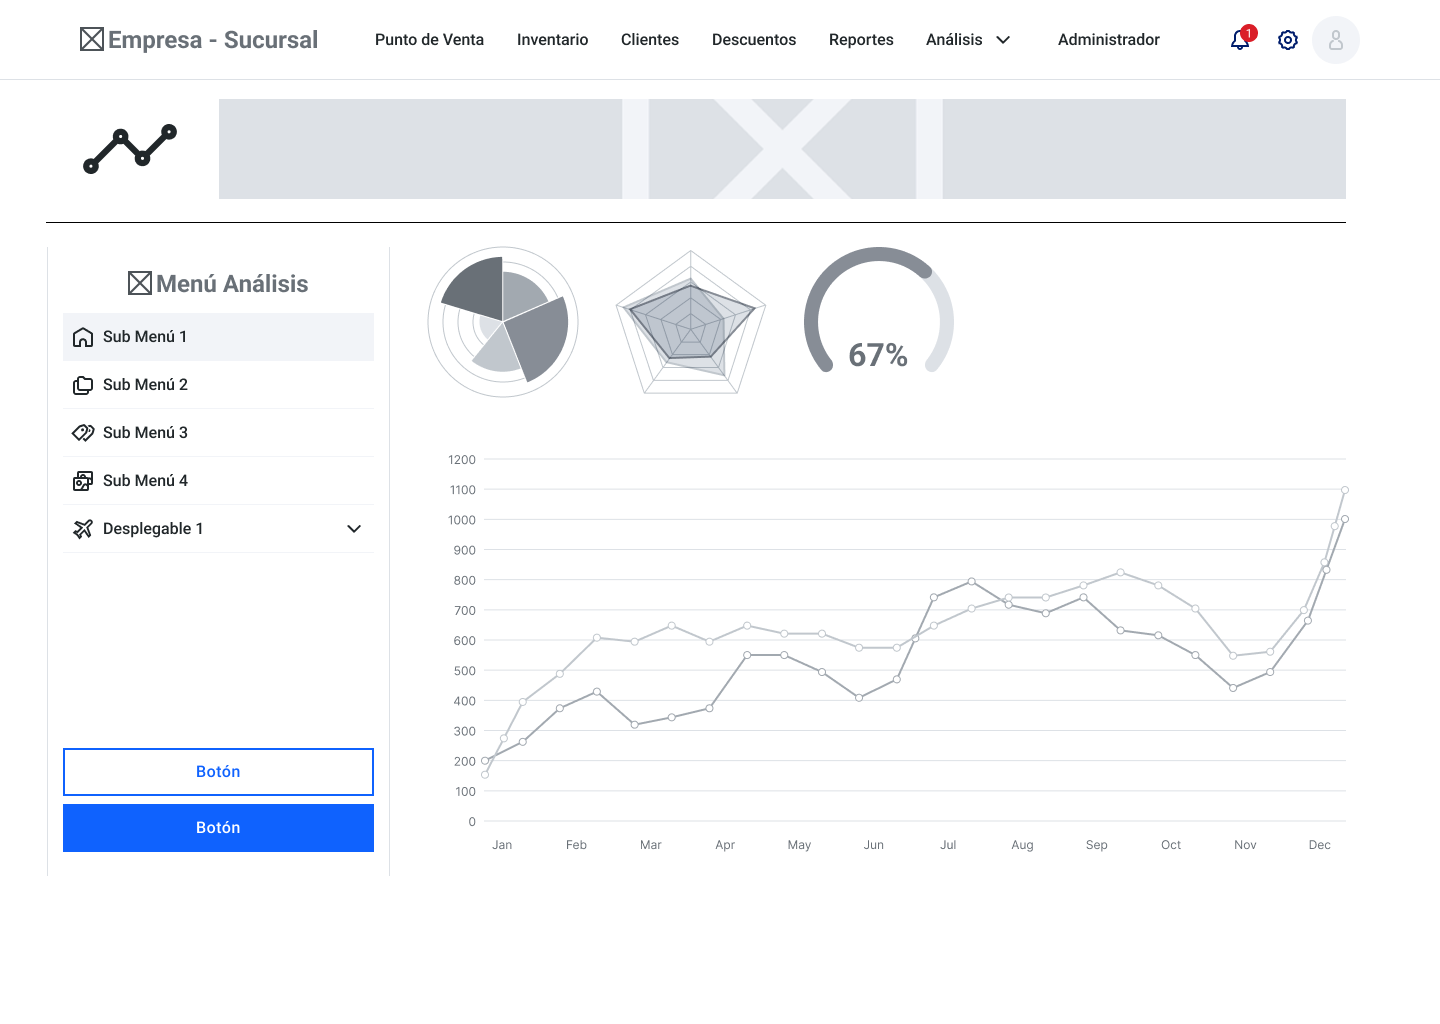
\includegraphics[scale=.4]{images/Analisis.png}
    \centering
    \caption{Página para la consulta de análisis y reportes en web y su vista correspondiente en Android.}
\end{figure}
